\subsubsection{Giao diện người dùng - Trang chủ}

Trang chủ của website cung cấp thông tin trực quan, đầy đủ về các công việc mới nhất như sau:

\begin{figure}[H]
    \centering
    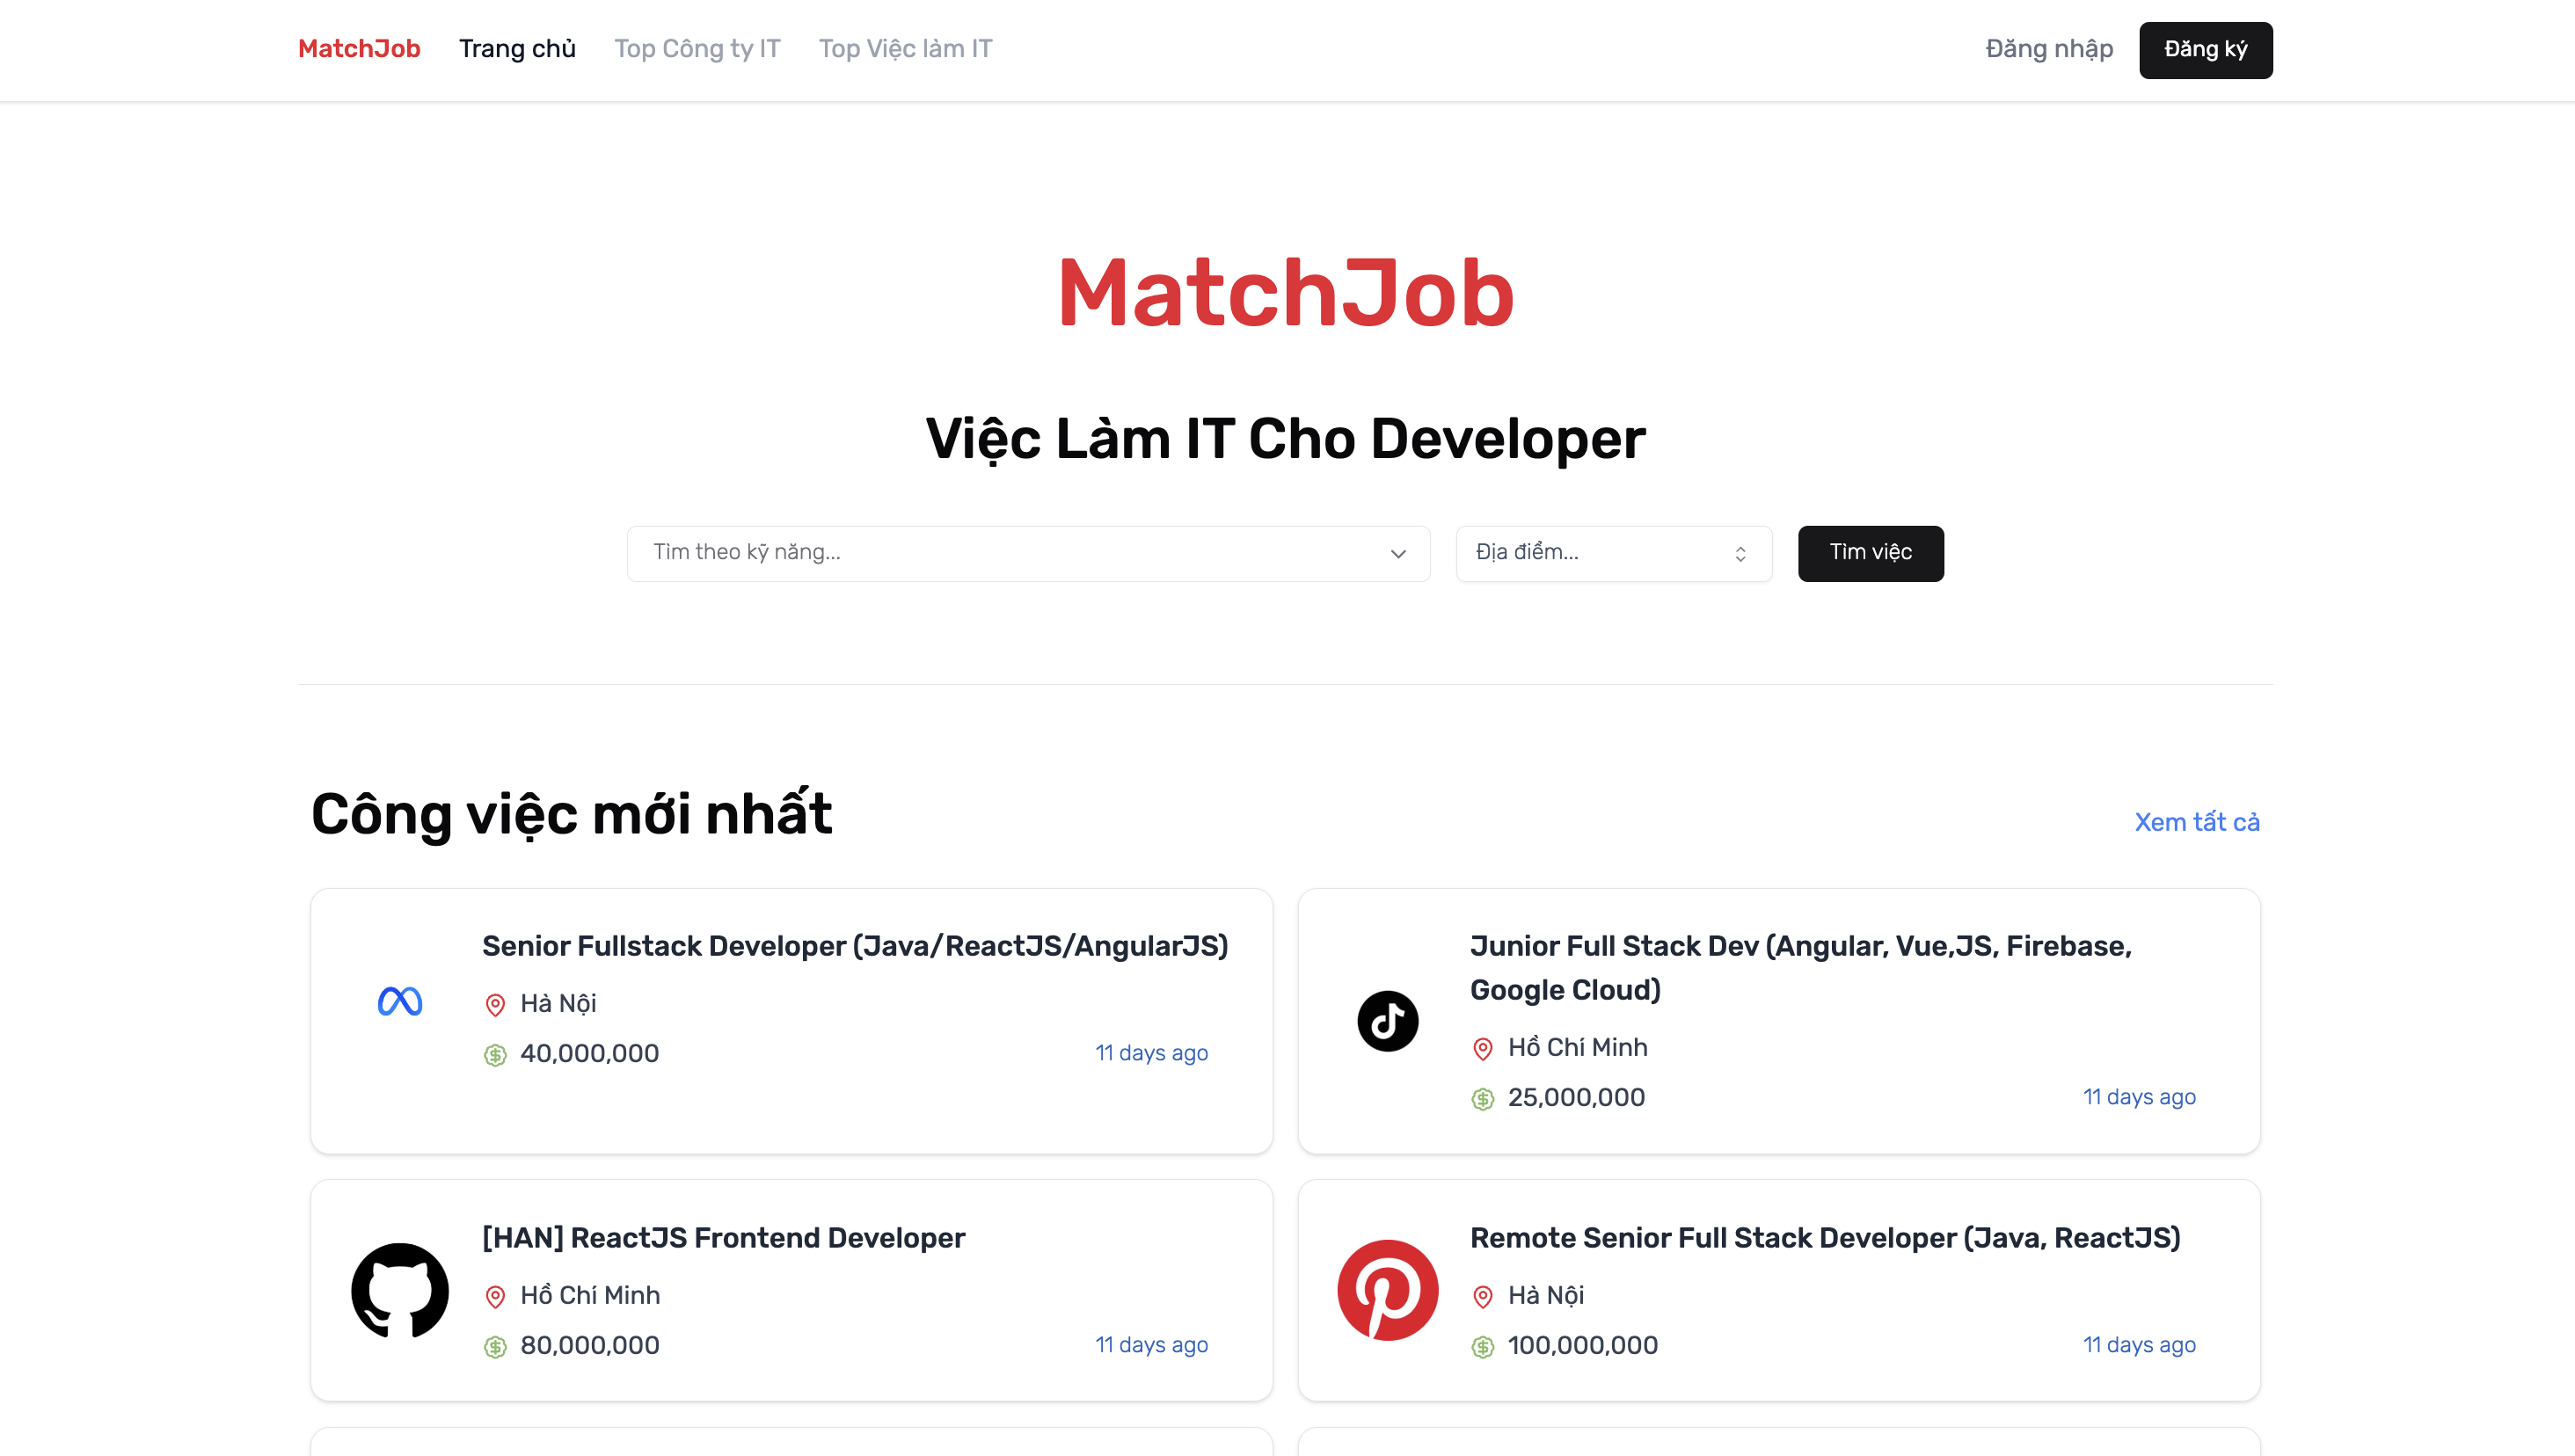
\includegraphics[width=\linewidth]{DBMS-Application/Images/user-screen-job.png}
    \caption{Trang chủ - Danh sách công việc đang tuyển dụng}
    \label{fig:homepage-job}
\end{figure}

Truy vấn sử dụng: \textbf{Query with composite condition}
\begin{lstlisting}
async findAll(current: number, pageSize: number, qs: string) {
    // Loc ra dieu kien filter va sort tu query parameters
    const { filter } = aqp(qs);

    // Truy van: Danh sach cong viec thoa man dieu kien filter
    const jobs = await this.db
      .collection('jobs')
      .find(filter)
      .skip((current - 1) * pageSize)
      .limit(pageSize)
      .toArray();

    // Tra ve response cho Frontend
    return jobs;
}
\end{lstlisting}

Giải thích:

\begin{enumerate}
    \item Frontend sẽ tự động gửi yêu cầu đến Backend thông qua API:
    \begin{lstlisting}[numbers=none]
GET /api/jobs?current=0&pageSize=6
    \end{lstlisting}
    
    \item Backend sẽ nhận được query parameters (\texttt{current} và \texttt{pageSize}) từ Frontend và thực hiện truy vấn CSDL với filter và phân trang:
    \begin{itemize}
        \item Sử dụng \texttt{find()} để lọc dữ liệu theo điều kiện \texttt{filter} (trong trường hợp này, \texttt{filter} là object rỗng (\texttt{\{\}}) nên sẽ trả về tất cả các công việc có trong hệ thống)
        \item Sử dụng \texttt{skip()} để bỏ qua các bản ghi không cần thiết
        \item Sử dụng \texttt{limit()} để giới hạn số lượng bản ghi trả về
    \end{itemize}

    \item Sau khi truy vấn được thực hiện thành công, Backend phản hồi danh sách các công việc cho Frontend để hiển thị lên giao diện người dùng
\end{enumerate}

Người dùng có thể tìm kiếm công việc bằng cách lọc theo \textbf{Địa điểm} và \textbf{Kỹ năng yêu cầu}. Ví dụ, tìm các công việc có yêu cầu kỹ năng \textbf{"React.JS"} và \textbf{"React Native"} tại \textbf{TP. Hồ Chí Minh}, hệ thống sẽ hiện lên một pop-up chứa các công việc thoả mãn.

\begin{figure}[H]
    \centering
    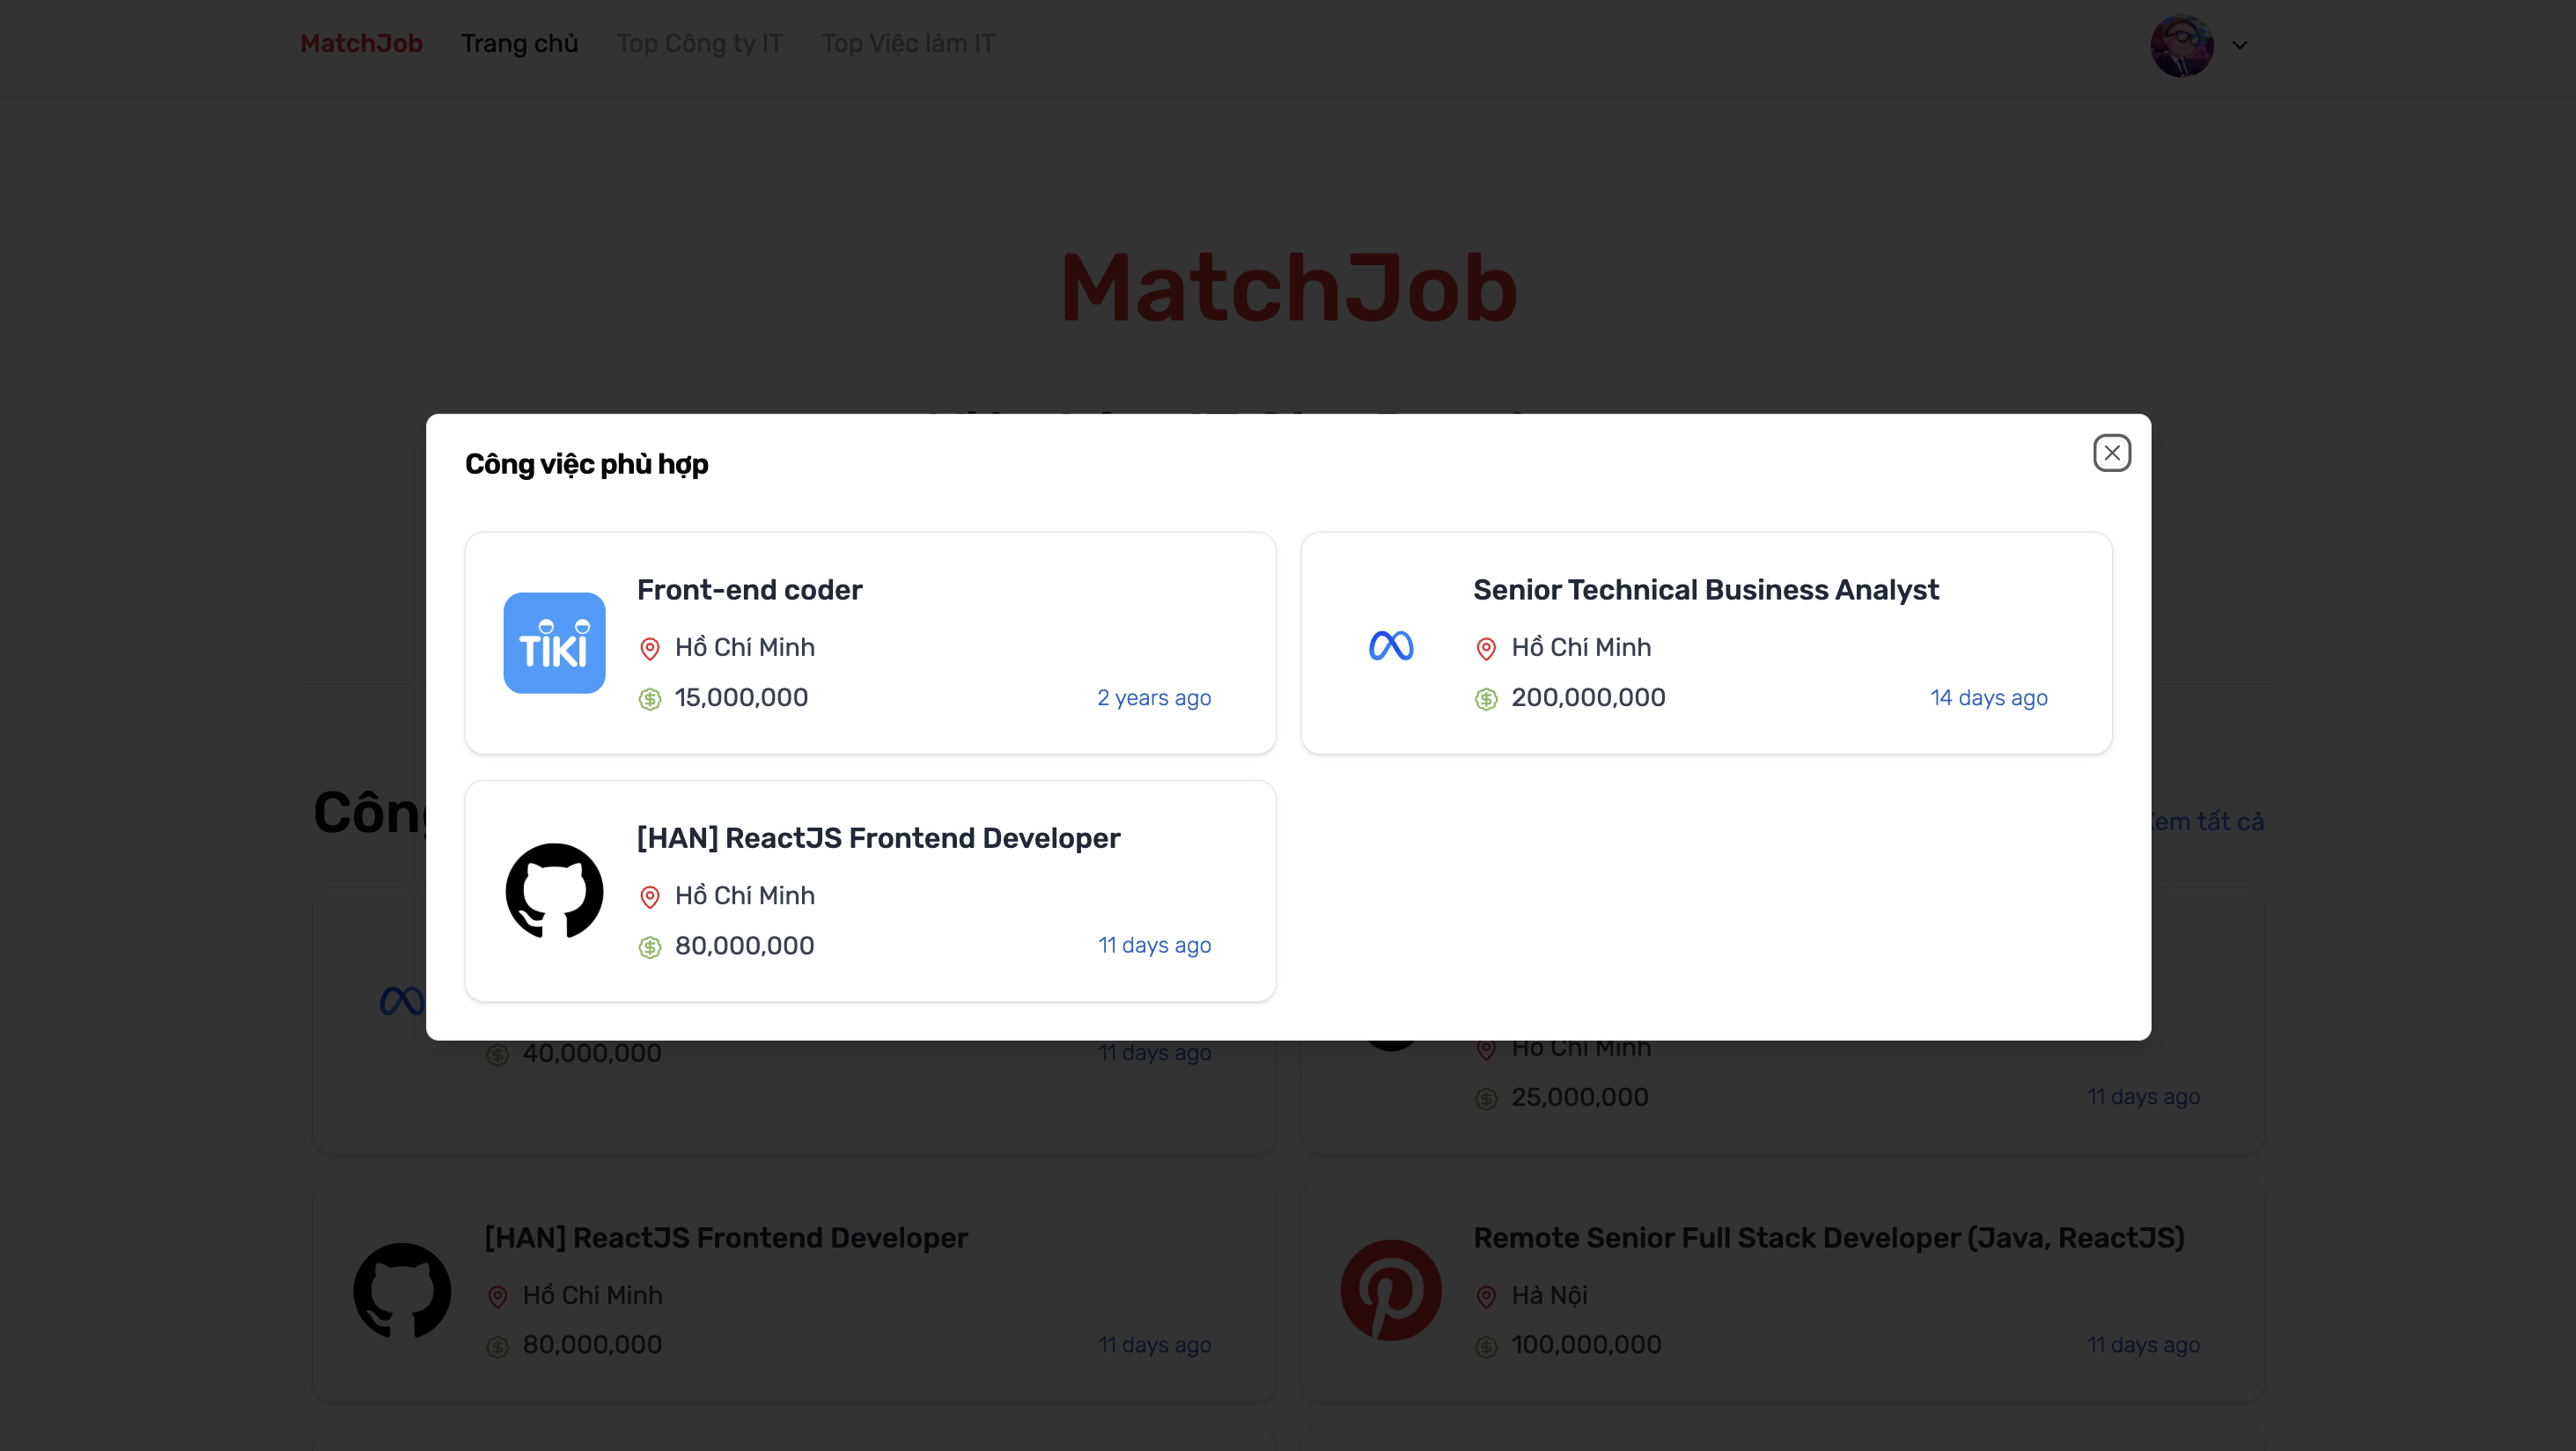
\includegraphics[width=\linewidth]{DBMS-Application/Images/modal-job-search.png}
    \caption{Trang chủ - Lọc công việc theo Địa điểm và Kỹ năng}
    \label{fig:homepage-job-search-filter}
\end{figure}

Truy vấn sử dụng: \textbf{Query with single/composite condition}

\begin{lstlisting}
async getJobsByLocationAndSkills(location: string, skills: string[]) {
    const query: { location?: string; skills?: { $in: string[] } } = {};

    if (location) query.location = location; 
    if (skills.length > 0) query.skills = { $in: skills }; 
    // query = { location: 'HOCHIMINH', skills: { $in: ['REACT.JS', 'REACT NATIVE'] } }

    // Truy van: Loc cac cong viec theo Ky nang va Dia diem
    return await this.db // Truy cap vao database he thong
    .collection('jobs')  // Truy cap vao collection 'jobs'
    .find(query)         // Loc theo dieu kien 'location' va 'skills' trong query
    .toArray();          // Chuyen ket qua ve dang mang
  }
\end{lstlisting}

Giải thích truy vấn:
\begin{itemize}
    \item Back-end nhận được yêu cầu từ Front-end, chứa 2 tham số \texttt{location} và \texttt{skills} trong query parameters và thực hiện xây dựng điều kiện lọc \texttt{query} với các giá trị đó
    
    Ví dụ: \texttt{ query = \{ location : ’HOCHIMINH’, skills : \{ \$in : [ ’REACT.JS’, ’REACT NATIVE’] \} \} }

    \item Sau đó, Back-end sẽ thực hiện truy vấn đến CSDL để lọc ra các công việc thoả mãn điều kiện vừa xây dựng được, và phản hồi về cho Front-end khi thành công
\end{itemize}

Người dùng cũng có thể xem được các công ty tuyển dụng hàng đầu cùng một số thông tin như: tên, logo công ty, số lượng công việc đang tuyển và thu thập cao nhất.

\begin{figure}[H]
    \centering
    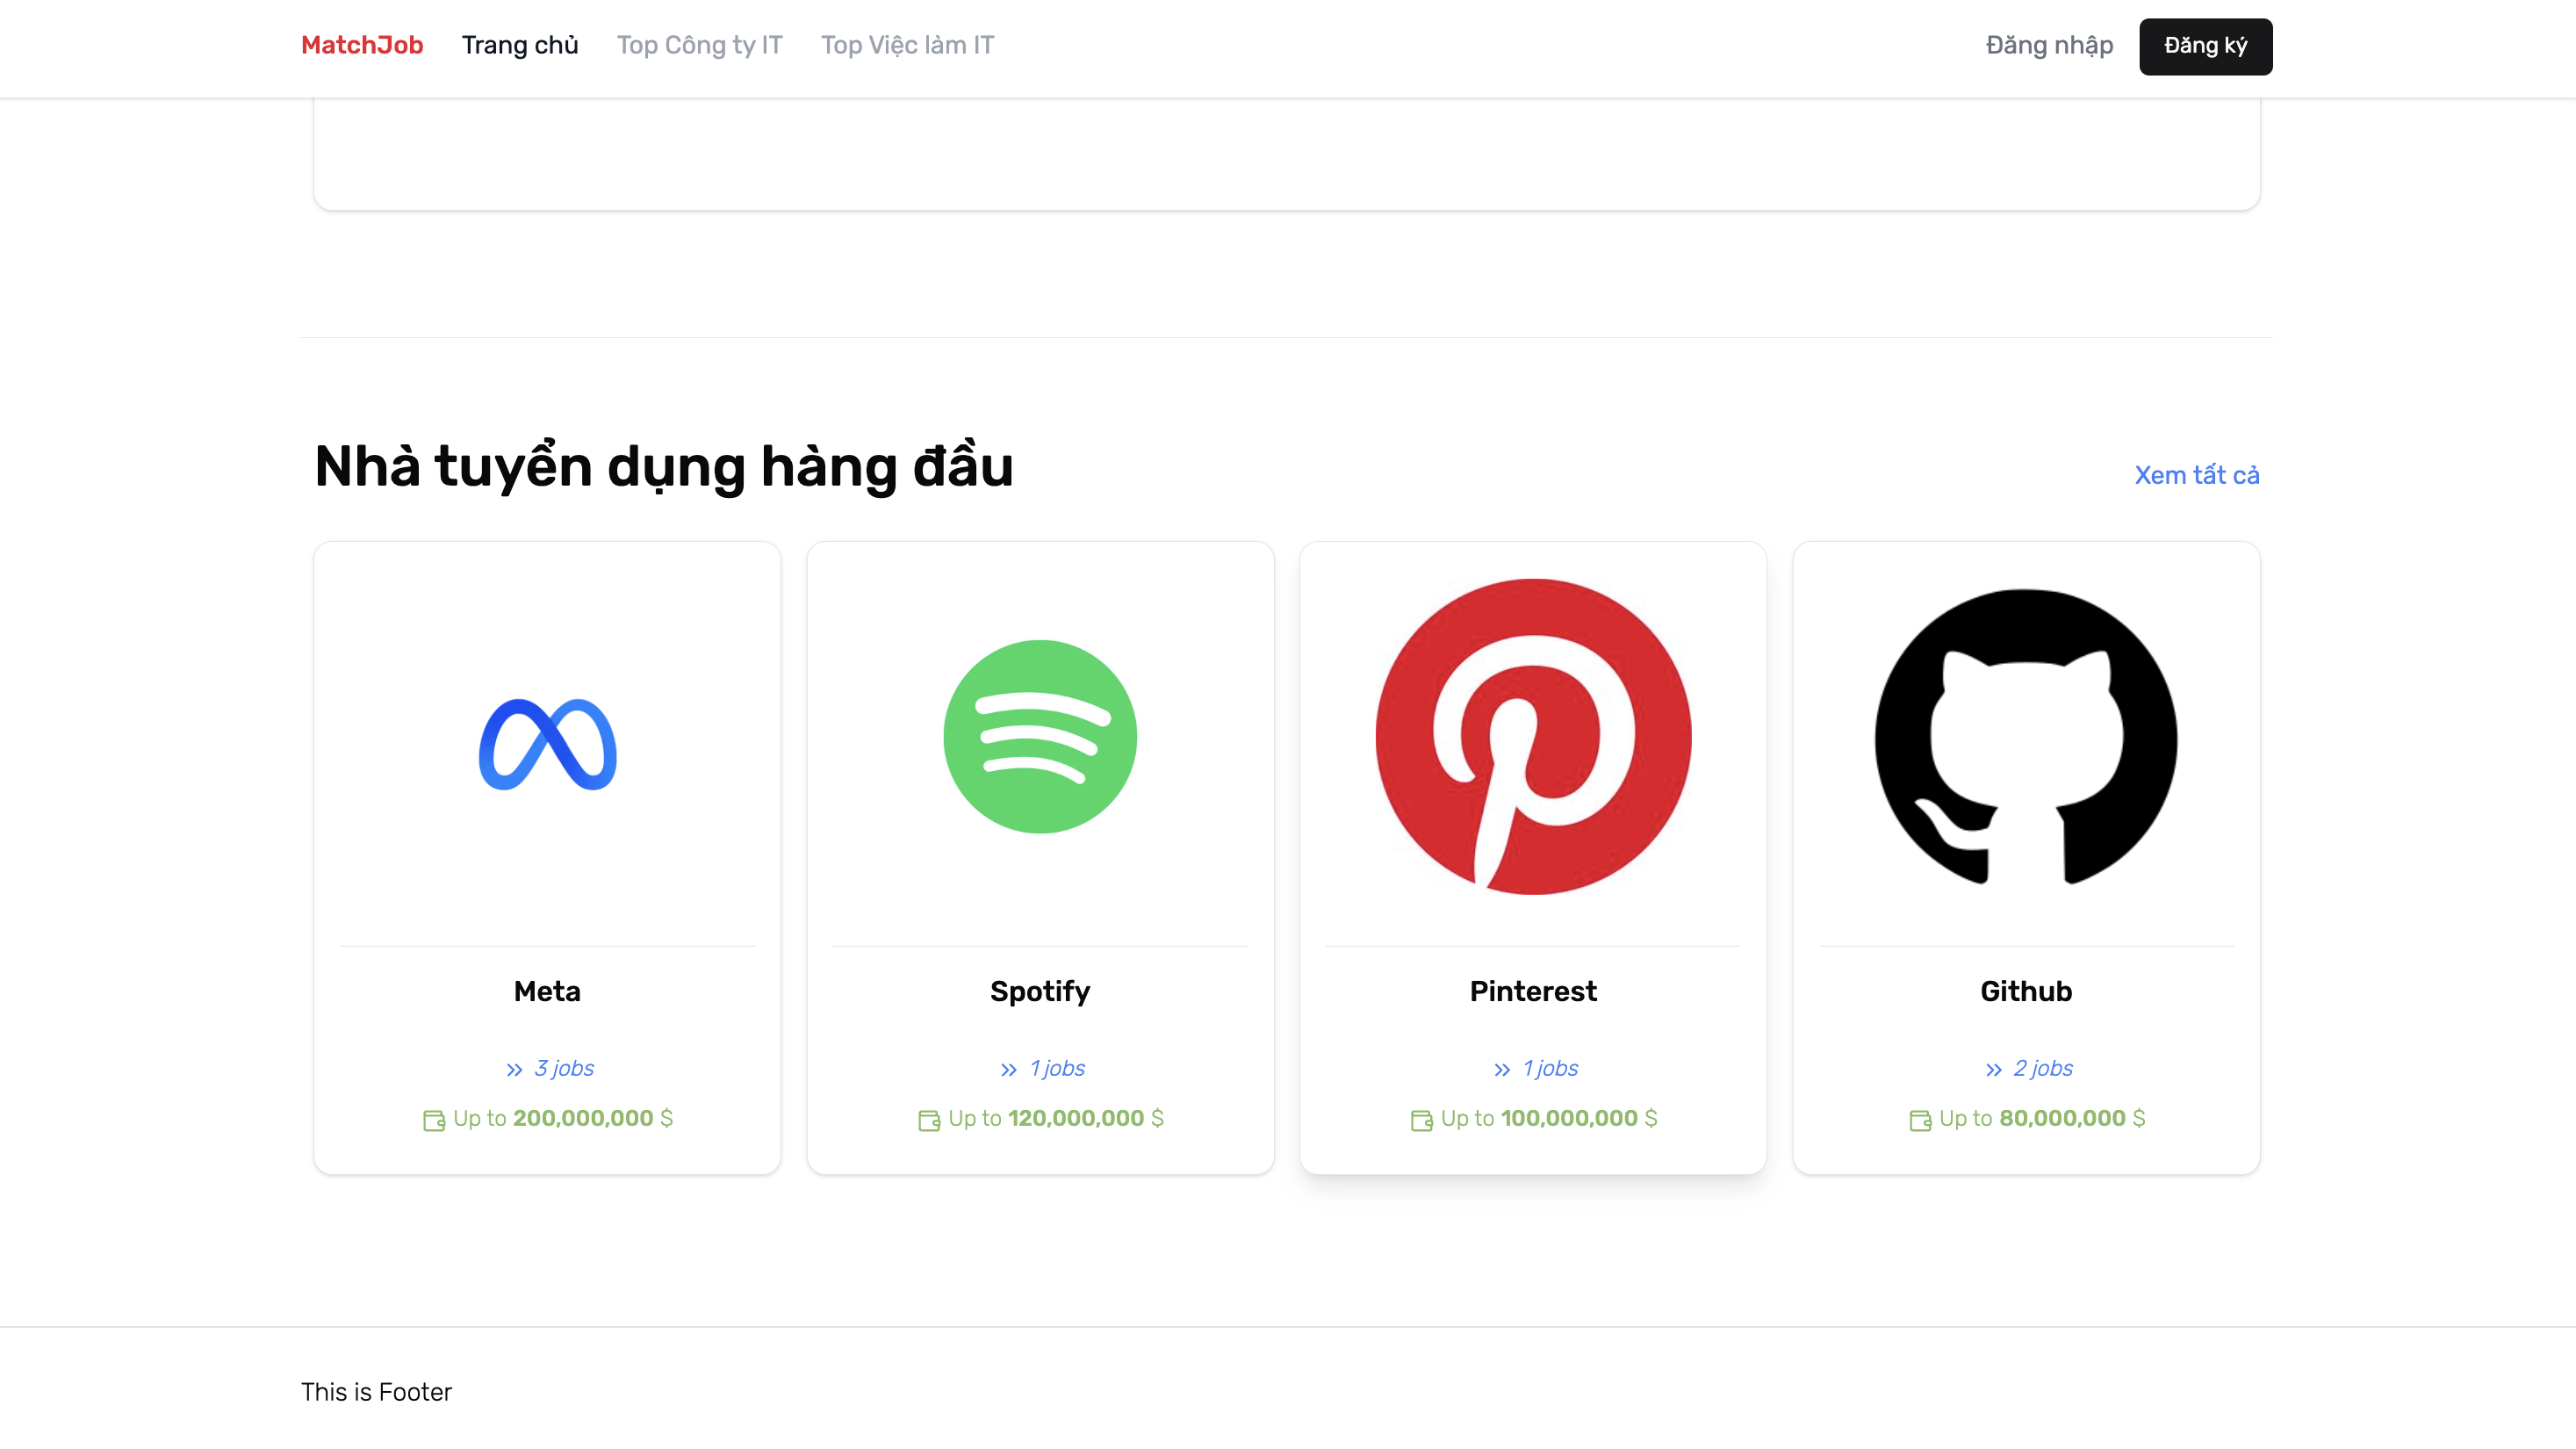
\includegraphics[width=\linewidth]{DBMS-Application/Images/user-screen-company.png}
    \caption{Trang chủ - Danh sách công ty tuyển dụng hàng đầu}
    \label{fig:homepage-company}
\end{figure}

Truy vấn sử dụng:
\begin{itemize}
    \item \textbf{Query with join}: Sử dụng và \texttt{\$lookup} để join collections \textbf{companies} với \textbf{jobs}
    \item \textbf{Query with aggregation functions}: Sử dụng \texttt{\$size}, \texttt{\$max}, \texttt{\$reduce} để tính toán số lượng công việc, mức lương cao nhất của công ty
\end{itemize}

\begin{lstlisting}
const pipeline = [
  { $match: filter },
  {
    $lookup: {
      from: 'jobs',
      let: { companyId: { $toString: '$_id' } },
      pipeline: [
        {
          $match: {
            $expr: {
              $eq: ['$company._id', '$$companyId'],
            },
          },
        },
      ],
      as: 'jobs',
    },
  },
  {
    $project: {
      _id: 1,
      name: 1,
      address: 1,
      description: 1,
      logo: 1,
      totalJobs: { $size: '$jobs' }, // Dem so luong cong viec
      maxSalary: { $max: '$jobs.salary' }, // Lay ra salary cao nhat
      maxSalaryJobId: {
        $reduce: {
          input: '$jobs',
          initialValue: null,
          in: {
            $cond: [
              { $eq: ['$$this.salary', { $max: '$jobs.salary' }] },
              '$$this._id',
              '$$value',
            ],
          },
        },
      },
    },
  },
  { $sort: { maxSalary: -1 } }, // Sap xep cong ty giam dan theo maxSalary
  { $skip: offset },
  { $limit: limit },
];

return await this.db
  .collection('companies')
  .aggregate(pipeline)
  .toArray();
\end{lstlisting}

Giải thích truy vấn: 
\begin{itemize}
    \item \texttt{\$match}: Lọc các công ty thỏa mãn điều kiện.
    \item \texttt{\$lookup}: Join collection \textbf{companies} (\texttt{\_id}) collection \textbf{jobs} (\texttt{companyId}) để lấy các công việc ứng với từng công ty
    \item \texttt{\$project}: Lọc ra các trường trong collection \textbf{companies} như \texttt{\_id}, \texttt{name}, \texttt{address}, \texttt{logo} và Tính toán các thông tin thống kê như số lượng công việc (\texttt{totalJobs}), lương cao nhất (\texttt{maxSalary}) và ID công việc có lương cao nhất (\texttt{maxSalaryJobId}) của từng công ty
    \item \texttt{\$sort}: Sắp xếp các công ty giảm dần theo lương cao nhất (\texttt{maxSalary})
    \item \texttt{\$skip} và \texttt{\$limit}: Phân trang kết quả
\end{itemize}

Bên cạnh đó, người dùng có thể xem nhanh thông tin các công việc đang tuyển dụng của một công ty cụ thể, thông qua các thẻ công ty được hiển thị:

\begin{figure}[H]
    \centering
    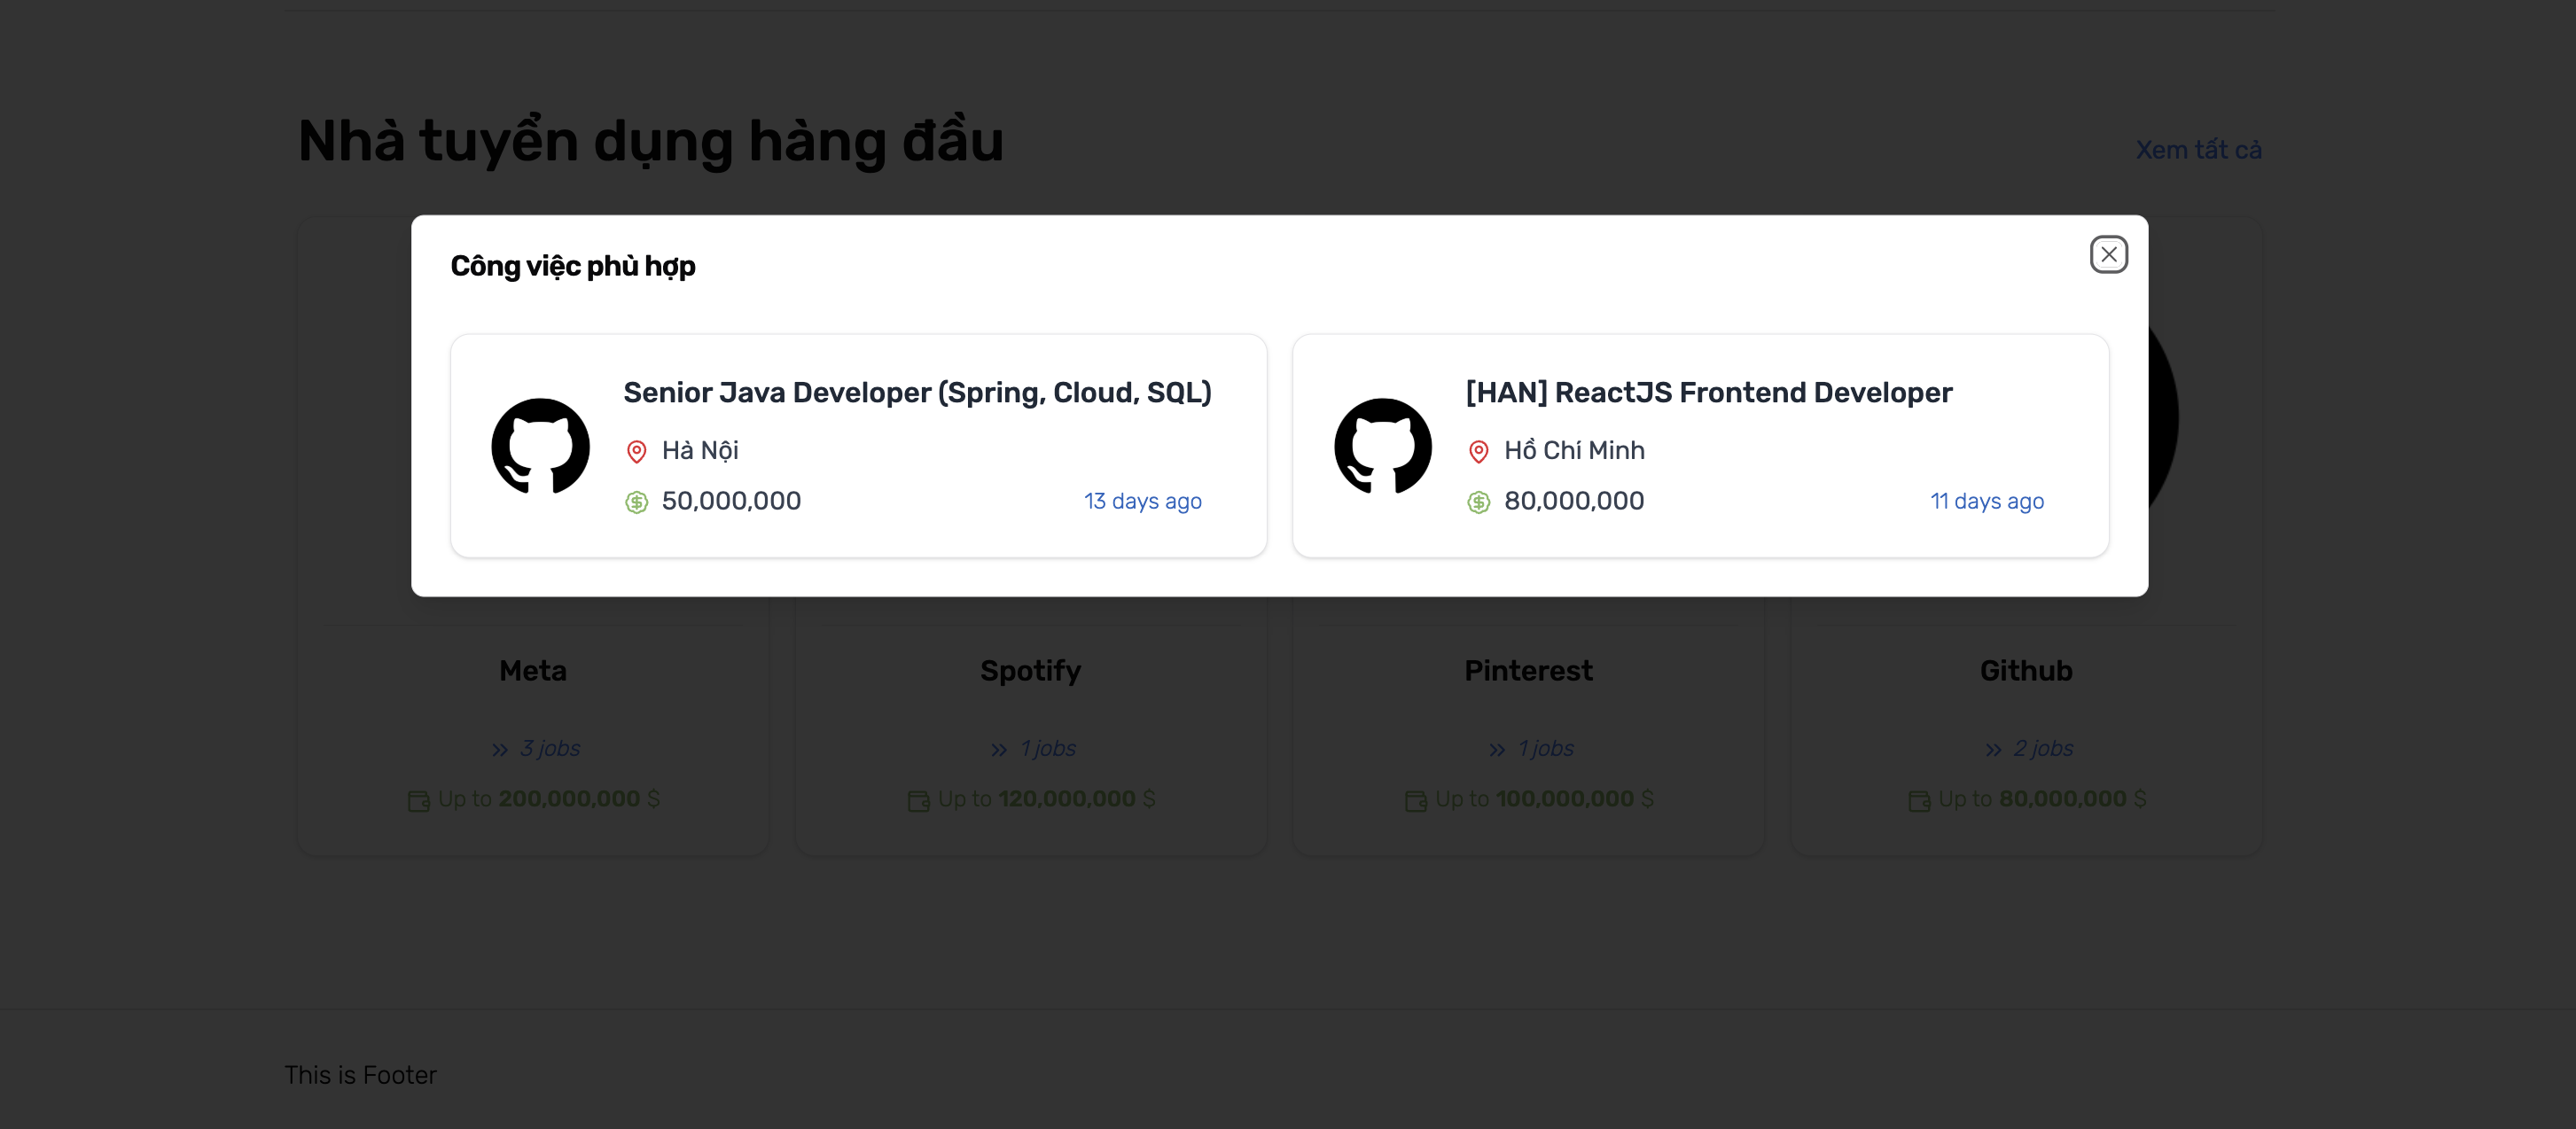
\includegraphics[width=\linewidth]{DBMS-Application/Images/modal-job-company.png}
    \caption{Trang chủ - Lọc ra các công việc thuộc một công ty cụ thể}
    \label{fig:homepage-job-company}
\end{figure}

Truy vấn sử dụng:
\begin{itemize}
    \item \textbf{Query with single condition}: Lọc document cụ thể từ collection \textbf{companies} dựa trên \texttt{\_id}

    \item \textbf{Query with join}: Thực hiện join giữa collection \textbf{companies} và \textbf{jobs} để lấy công việc liên quan
\end{itemize}

\begin{lstlisting}
const pipeline = [
  {
    $match: { _id: new ObjectId(companyId) }, // Loc ra cong ty co _id = companyId duoc truyen vao
  },
  {
    $lookup: {
      from: 'jobs', // Join collection 'companies' voi collection 'jobs'
      let: { companyId: { $toString: '$_id' } },
      pipeline: [
        {
          $match: {
            $expr: { $eq: ['$company._id', '$$companyId'] },
          },
        },
      ],
      as: 'jobs', // Luu ket qua vao field 'jobs' cho tung cong ty
    },
  },
  {
    $project: { // Loc ra cac field can thiet
      _id: 1,
      name: 1,
      address: 1,
      description: 1,
      logo: 1,
      jobs: 1,
    },
  },
];

return await this.db
  .collection('companies')
  .aggregate(pipeline)
  .toArray();
\end{lstlisting}

Giải thích truy vấn:
\begin{itemize}
    \item \texttt{\$match}: Lọc công ty cụ thể từ collection companies dựa trên \texttt{\_id} được truyền vào (\texttt{companyId}).
    
    \item \texttt{\$lookup}: Join collection \textbf{companies} với collection \textbf{jobs} để tìm tất cả các công việc thuộc công ty đó, bằng cách so sánh \texttt{\_id} của công ty trong \textbf{companies} với \texttt{company.\_id} trong \textbf{jobs} và lưu danh sách công việc vào trường \textbf{jobs}.


    \item \texttt{\$project}: Chọn các trường cần trả về gồm \texttt{\_id}, \texttt{name}, \texttt{address}, \texttt{description}, \texttt{logo}, và \texttt{jobs}.
\end{itemize}

Cuối cùng, người dùng có thể xem thống kê các kỹ năng có nhu cầu tuyển dụng nhiều, được thu thập từ các công việc đang được tuyển dụng:

\begin{figure}[H]
    \centering
    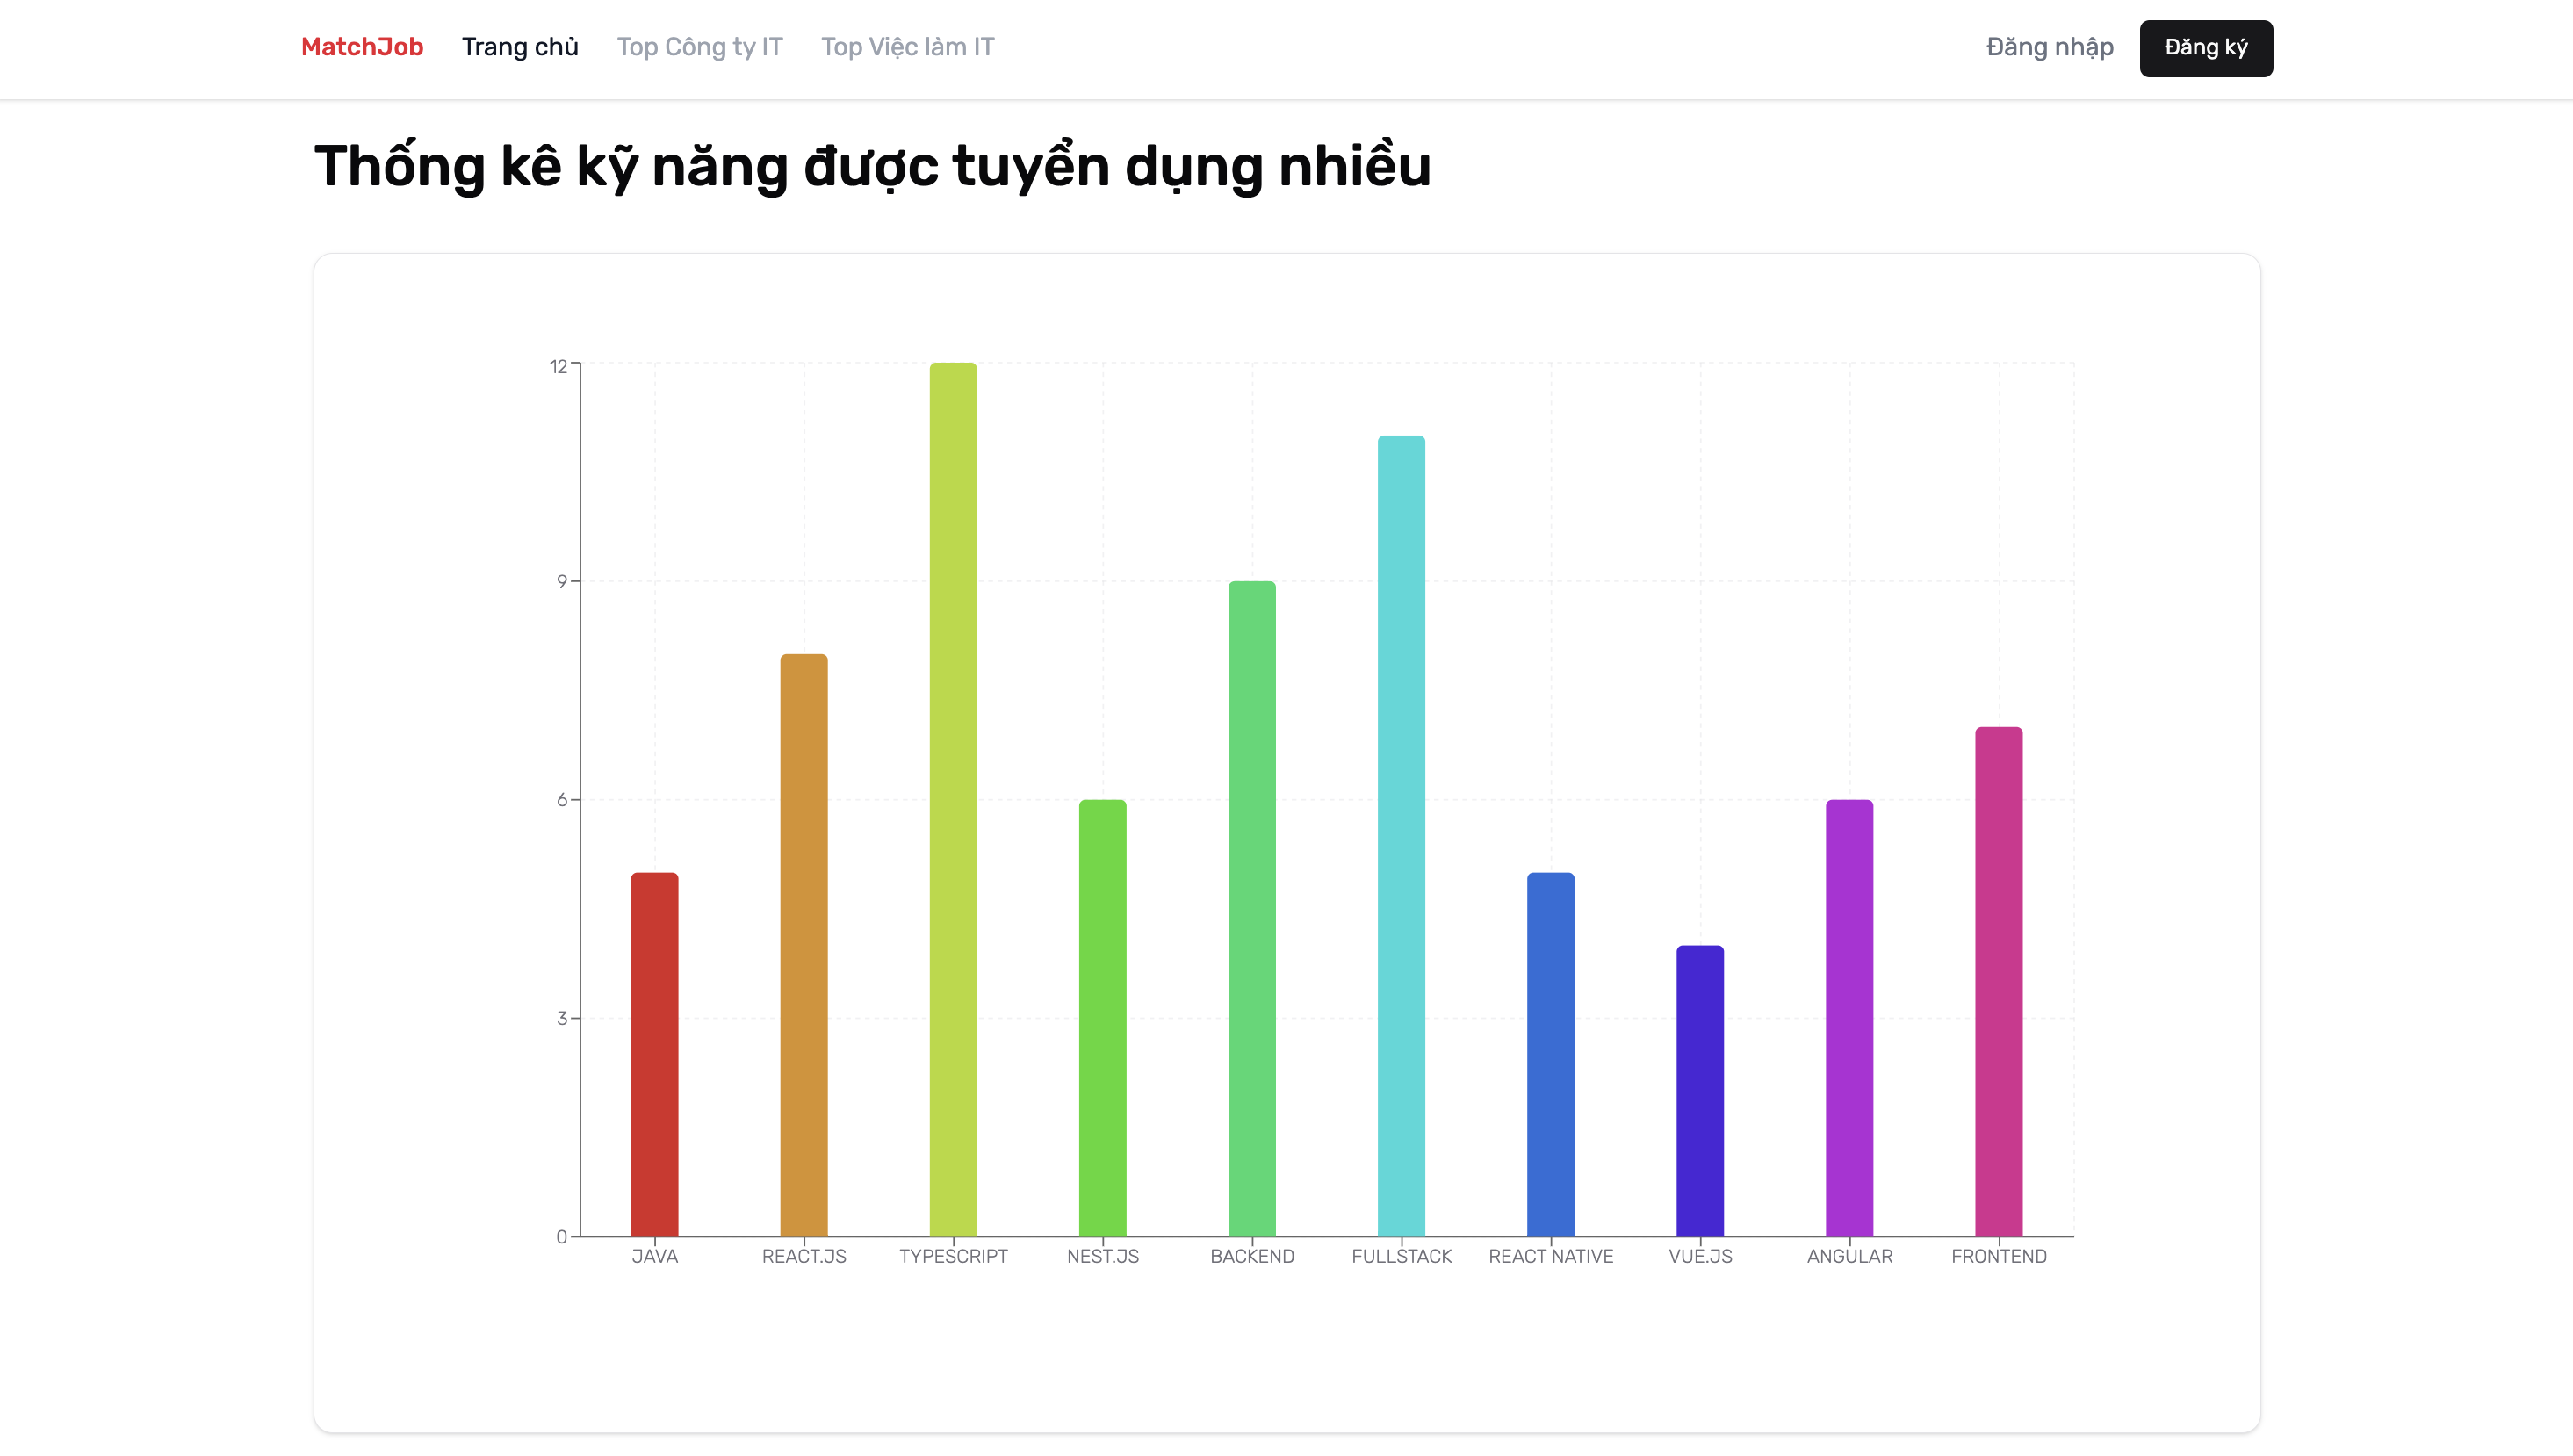
\includegraphics[width=\linewidth]{DBMS-Application/Images/user-screen-skill-stats.png}
    \caption{Trang chủ - Thống kê kỹ năng được tuyển dụng nhiều}
    \label{fig:enter-label}
\end{figure}

Truy vấn sử dụng: \textbf{Query with aggregation functions} - Sử dụng \texttt{\$sum} để tính tổng số công việc yêu cầu từng kỹ năng.

\begin{lstlisting}
const pipeline = [
  { $unwind: '$skills' },
  { $group: { _id: '$skills', total: { $sum: 1 } } },
  { $project: { skill: '$_id', total: 1, _id: 0 } },
];

return await this.db
  .collection('jobs')
  .aggregate(pipeline)
  .toArray();
\end{lstlisting}

Giải thích truy vấn:
\begin{itemize}
    \item \texttt{\$unwind}: Tách từng phần tử trong mảng skills của mỗi công việc thành các document riêng lẻ.
    \item \texttt{\$group}: Nhóm các document theo kỹ năng (skills) và đếm số lượng công việc yêu cầu kỹ năng đó bằng cách cộng dồn (\$sum: 1).
    \item \texttt{\$project}: Chọn các trường cần trả về, đổi tên \_id thành skill và bỏ trường \_id trong kết quả.
\end{itemize}